%label:"fig:LagrangiansInTheFukayaSeidelCategory"
%type:"figure"
%name:"Lagrangians in the Fukaya Seidel Category"
%caption:"A Lagrangian submanifold in a Fukaya-Seidel category needs to have prescribed behavior going off to infinity."
%parent:"art_ASideLandauGinzburgModel"


    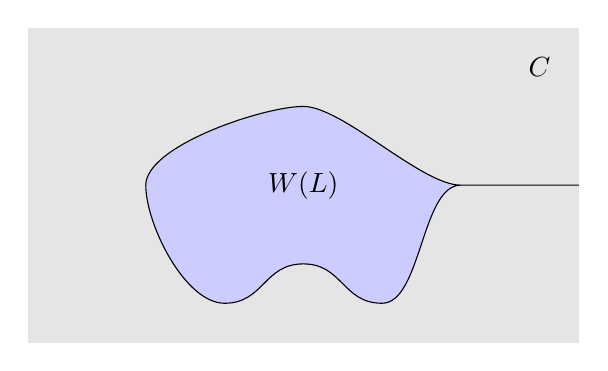
\begin{tikzpicture}

        \fill[gray!20] (-3,2.5) rectangle (4,-1.5);
        \draw[fill=blue!20] (2.5,0.5) .. controls (2,0.5) and (1,1.5) .. (0.5,1.5) .. controls (0,1.5) and (-1.5,1) .. (-1.5,0.5) .. controls (-1.5,0) and (-1,-1) .. (-0.5,-1) .. controls (0,-1) and (0,-0.5) .. (0.5,-0.5) .. controls (1,-0.5) and (1,-1) .. (1.5,-1) .. controls (2,-1) and (2,0.5) .. (2.5,0.5) .. controls (4,0.5) and (3,0.5) .. (4,0.5);
        \node at (0.5,0.5) {$W(L)$ };
        \node at (3.5,2) {$\mathbb{C}$};
    \end{tikzpicture}

